\Chapter{Étude de plasmas magnétisés}
\chaptermark{Étude de plasmas magnétisés}
\begin{refsection}
Ce quatrième chapitre porte sur l'étude de deux cas concrets,
chacun représentatif d'une configuration magnétique particulière : le filtre
magnétique avec le propulseur PEGASES et la colonne de plasma magnétisée de la
source d'ions négatifs CYBELE. 
A travers ces exemples, nous testons les possibilités du nouveau code MAGNIS,
tout en explorant la physique qu'il révèle. Les simulations sont discutées et
confrontées aux mesures expérimentales ainsi qu'aux résultats de modèles
statistiques.
En fin de chapitre, nous simulons une configuration typique de bord de tokamak,
de champ magnétique intense et où le transport est principalement de nature
turbulente. 
		 
\section{Barrière magnétique - PEGASES}
PEGASES, acronyme de \emph{Plasma Propulsion with Electronegative Gases}, est
un prototype de propulseur électrostatique à grille (PEG)
ion-ion\parencite{Chabert} conçu au LPP (Laboratoire de Physique des
Plasma) de l'Ecole Polytechnique de Paris et qui a pour originalité d'éjecter à
la fois des ions négatifs et des ions positifs pour générer la poussée. Dans ce
nouveau concept prometteur, les faisceaux d'ions de charges opposées se
neutralisent mutuellement à la sortie du propulseur, rendant la cathode
neutralisante non nécéssaire. Contrairement aux Propulseurs à Effets Hall
\footnote{Les propulseurs ioniques classiques, Propulseurs à Effet Hall (PEH),
sont constitués de trois étages : la source d'ion, l'étage d'accélération, où un
fort champ électromagnétique accélère les ions, et une cathode pour neutraliser
les ions positifs et éviter que le propulseur ne se charge.}, les PEG n'ont
donc pas de séparation entre les étages de création et d'accélération des ions.
Pour filtrer les électrons chauds et favoriser la création du plasma ion-ion, une
barrière magnétique d'une centaine de Gauss est placée entre la zone
d'ionisation et la région d'extraction.

\begin{figure}[htbp]
\centering
\includegraphics[width=0.75\textwidth]{figures/4-pegases3D.png}
{\caption{Schéma de principe de fonctiopnnement du propulseur PEGASES avec les
différents étages mentionnés en italiques\parencite{Popelier}.}
\label{4-pegases3D}}
\end{figure}

La structure en différents étages de PEGASES est représentée sur la
figure \ref{4-pegases3D}. Dans le premier étage, un gaz électronégatif est
excité inductivement par une puissance RF.
Le plasma de la source, consitué d'ion positifs, d'ions négatifs et d'électrons
est ensuite filtré par une barrière magnétique dans le deuxième étage du
propulseur. L'intensité de la barrière magnétique est choisie de façon à ce que
seuls les électrons soient magnétisés, laissant les ions diffuser librement à
travers le champ. Le plasma se sépare ainsi en deux régions de températures
électroniques différentes, l'une chaude du côté de l'injection de puissance,
l'autre plus froide en aval de la barrière, où se forme un plasma
ion-ion. Le troisième étage est enfin constitué du plasma ion-ion et
d'une série de grille que l'on polarise pour extraire et accélérer les
particules, afin de former les faisceaux d'ions qui feront la poussée. La grille
d'extraction est la seule paroi conductrice du propulseur, ce qui permet de
contrôler le potentiel plasma en s'affranchissant du problème de l'état de
surface et de la contamination des parois.

La source ICP est entretenue à 4MHz avec une bobine plane dopée par un noyau de
ferrite protégée d'une fine (3mm) couche de céramique\parencite{Godyak} qui
peut fournir de 50W à 250W.
La géométrie de la source et la configuration du
filtre magnétique ont été choisies d'après les résultats de Aanesland \emph{et
al.}\parencite{Aanesland} qui donne les conditions nécéssaires à la
formation d'un plasma ion-ion. L'enceinte du propulseur, de dimension
12x12x8cm, est usiné à partir d'un bloc d'aluminium, anodisée afin de rendre
ses parois diélectriques. Une autre version, constituée de paroi conductrices,
est aussi utilisée à des fins de diagnostique de la source.

Bien que MAGNIS ne puisse pas encore simuler les plasmas électronégatifs qui
nécéssitent une description des intéractions chimiques, il peut être utilisé
pour caractériser le transport complexe des électrons et du plasma en général à
travers le filtre magnétique. Pour étudier ce comportement, nous choisissons de
simuler un plasma d'argon, avec la géométrie présentée figure
\ref{4-pegasesSimDomain} :
\begin{figure}[htbp]
\centering
\includegraphics[width=0.6\textwidth]{figures/4-pegasesSimDomain.png}
{\caption{Le domaine de simulation est le plan perpendiculaire au champ
magnétique.}
\label{4-pegasesSimDomain}}
\end{figure}

Rectangulaire et de
dimension similaire à celle du prototype, la puissance est déposée dans la
région en amont du filtre magnétique sous la forme d'une demi-gaussienne de 2cm
de largeur. Le filtre magnétique est aussi de forme gaussienne, centré en
x=7.5cm et de largeur $\sim$ 2.5cm. Les parois seront choisies
conductrices ou diélectriques, avec une polarisation éventuelle de la grille
d'extraction (en jaune à droite du domaine). La puissance totale absorbée et la
densité de gaz sont fixées respectivement à 150W et 1mTorr.

Le type de solutions obtenues par MAGNIS dans le cas de parois diélectriques et
sans bias appliqué sont illustrées figure \ref{2-CartesWithTe} :

\begin{figure}[htbp]
    \centering
    \subfigure[]{\label{4-PegasesCarteDensiteBase}
    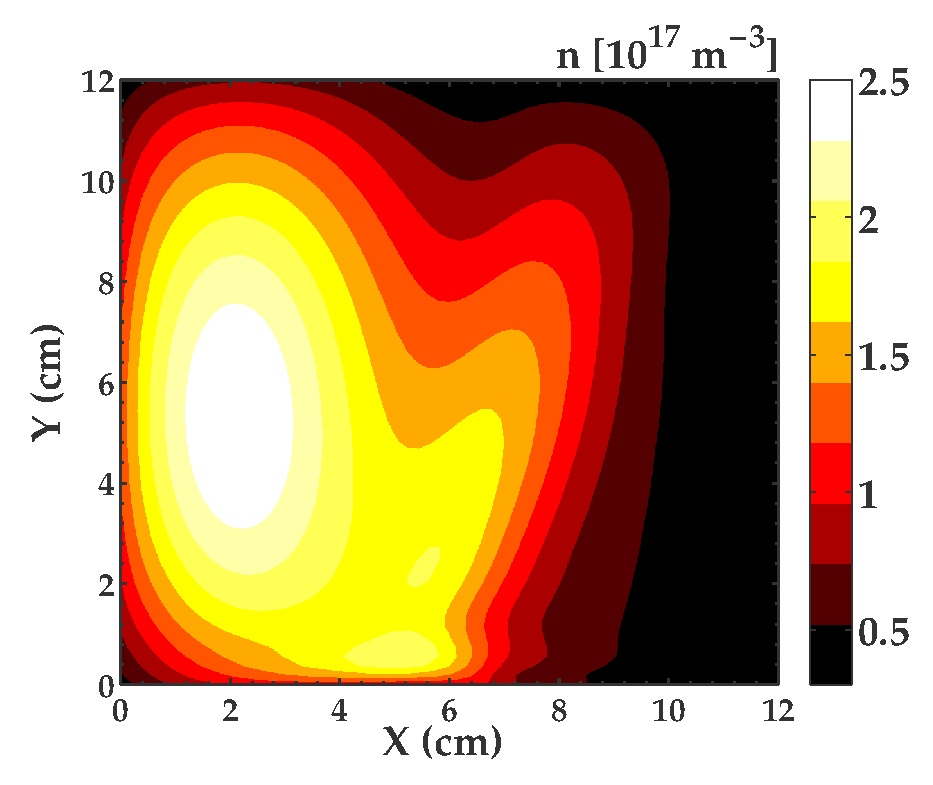
\includegraphics[height=5.75cm]{figures/4-PegasesCarteDensiteBase.eps}}
    \subfigure[]{\label{4-PegasesCartePotentielBase}
    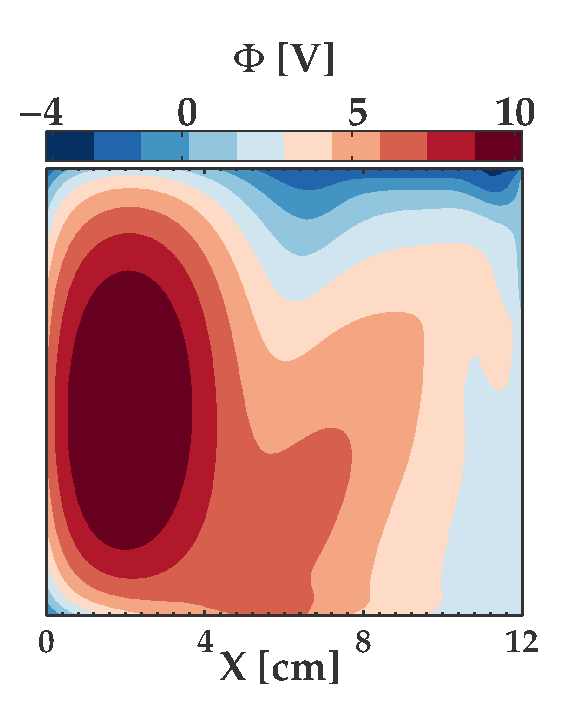
\includegraphics[height=5.75cm]{figures/4-PegasesCartePotentielBase.eps}}
    \subfigure[]{\label{4-PegasesCarteTemperatureBase}
    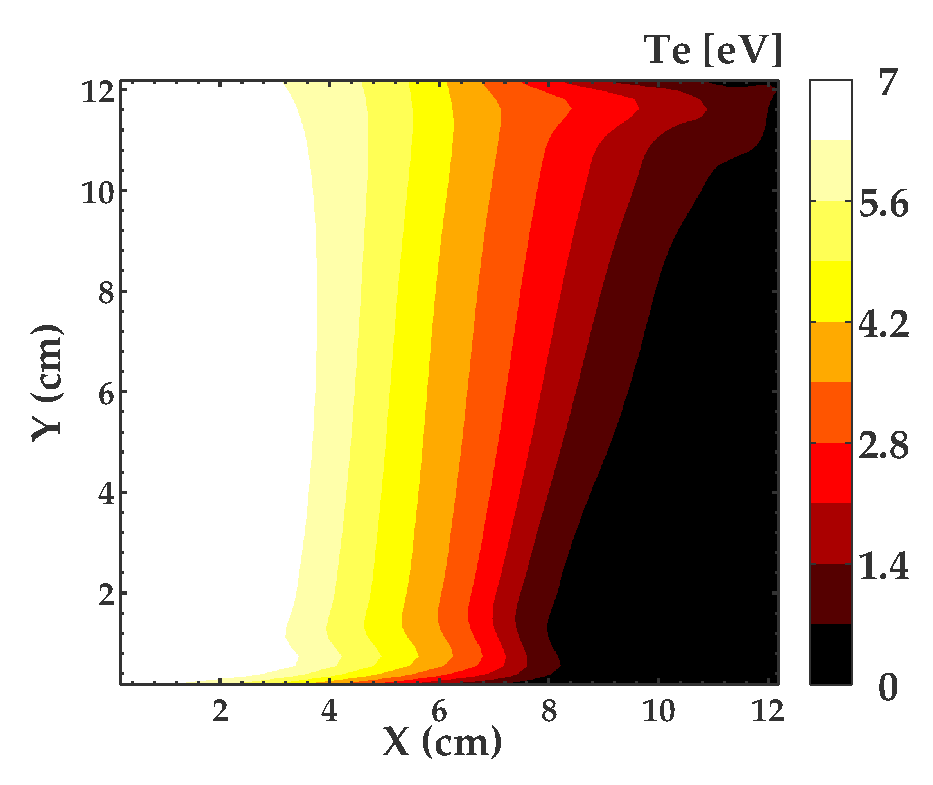
\includegraphics[height=5.75cm]{figures/4-PegasesCarteTemperatureBase.eps}}
    \caption{Cartes de densité \subref{4-PegasesCarteDensiteBase}~, de potentiel
    \subref{4-PegasesCartePotentielBase}~ et de température
    \subref{4-PegasesCarteTemperatureBase} dans le cas de parois diélectriques.}
    \label{2-CartesWithTe}
	\end{figure}

La densité maximum de la source, 2.5x10$^{17}\text{m}^{-3}$  est atteinte au
centre de la région d'ionisation. La densité du plasma décroît ensuite très
rapidement sur une longueur de 2 à 4cm. On peut observer de plus qu'une partie
du plasma diffuse en travers du champ magnétique. Le potentiel électrique, qui
suit le profile de densité, donne naissance à un champ électrique d'une centaine
de Volt par mètre, quasiment ambipolaire dans la région non magnétisée, et
plutôt faible dans le filtre magnétique.

\begin{figure}[htbp]
  \centering
    \subfigure[]{\label{4-PegasesCarteFluxEBase}
    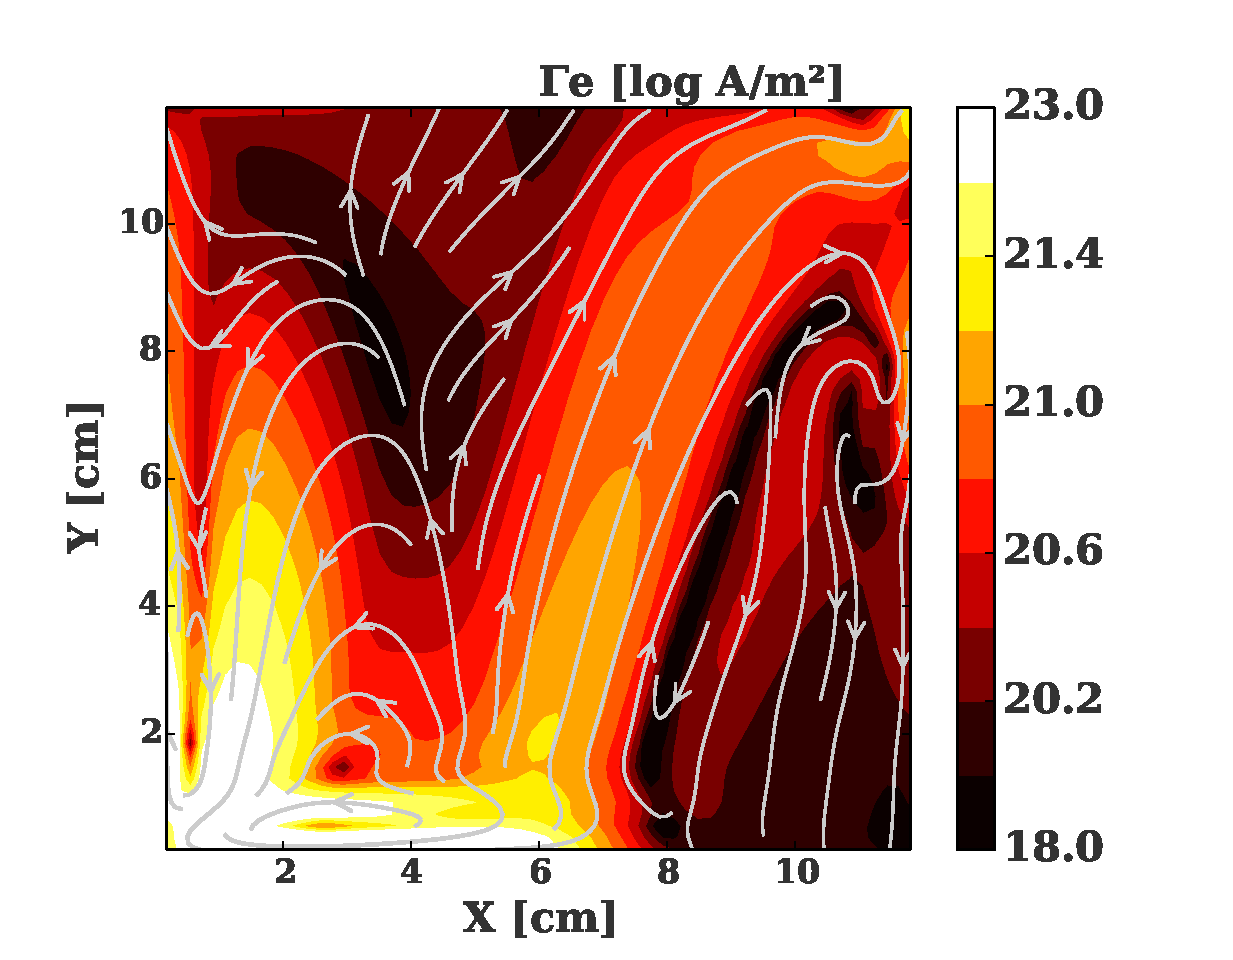
\includegraphics[height=4cm]{figures/4-PegasesCarteFluxEBase.eps}}
    \subfigure[]{\label{4-PegasesCarteFluxIBase}
    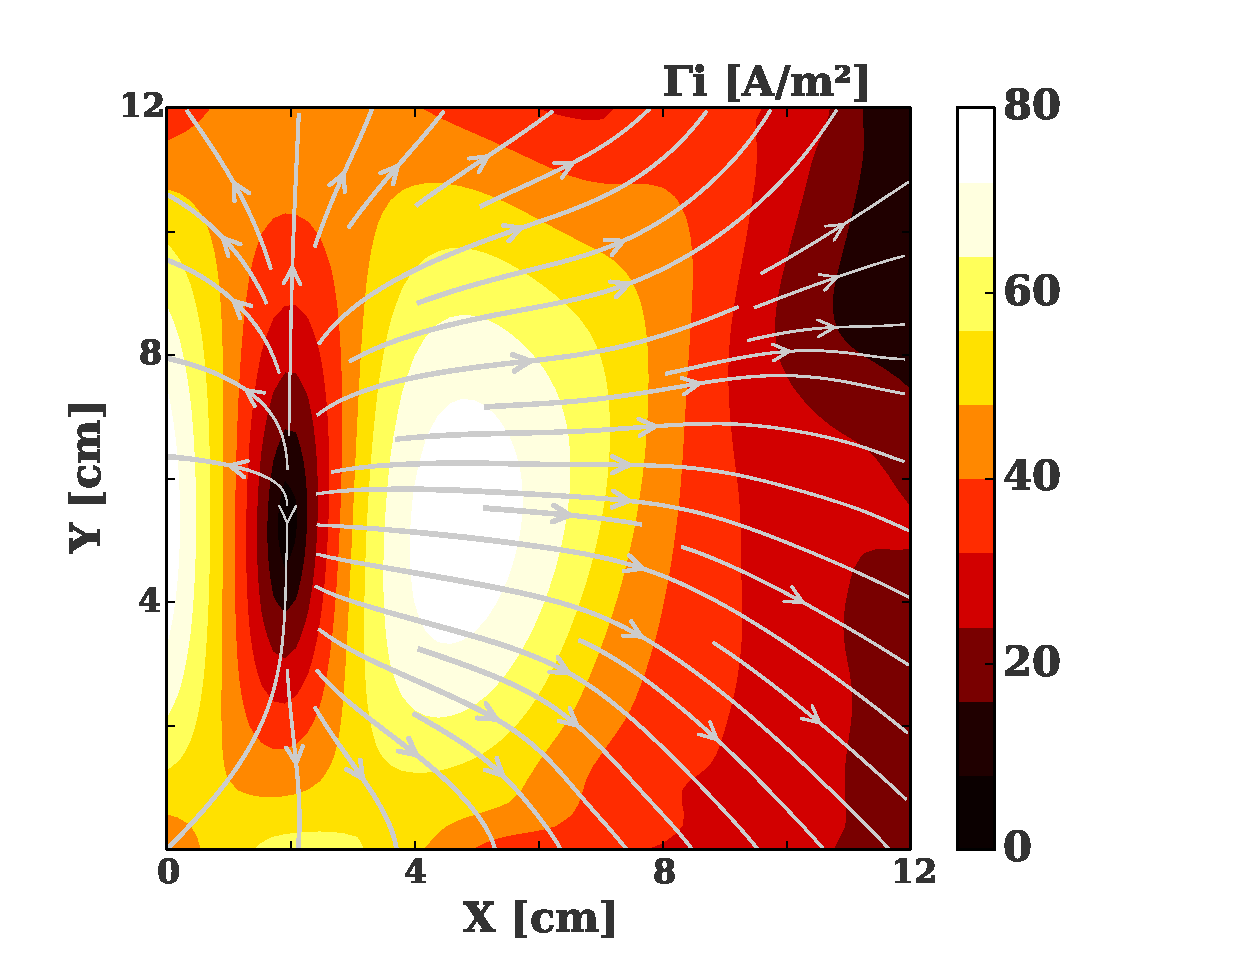
\includegraphics[height=4cm]{figures/4-PegasesCarteFluxIBase.eps}}
    \caption{Cartes de densité\subref{4-PegasesCarteFluxEBase}~, de
    potentiel\subref{4-PegasesCarteFluxEBase}~ et de
    température\subref{4-PegasesCarteFluxEBase}}
    \label{pandas}
\end{figure}
\subsection{Comparaison expérimentale}

a
	
	\subsubsection{Scan en pression}
	\begin{figure}[htbp]
  \centering
    \subfigure[]{\label{4-pegasesCompPressDenProfile}
    
\includegraphics[height=4cm]{figures/4-pegasesCompPressDenProfile.eps}}
    \subfigure[]{\label{4-pegasesCompPressTempProfile}
    
\includegraphics[height=4cm]{figures/4-pegasesCompPressTempProfile.eps}}
    \caption{Cartes de densité\subref{4-pegasesCompPressTempProfile}~, de
    potentiel\subref{4-pegasesCompPressTempProfile}~ et de
    température\subref{4-pegasesCompPressTempProfile}}
    \label{pandas}
\end{figure}
	\subsubsection{Variations du champ magnétique}

a
	
	\begin{figure}[htbp]
  \centering
    \subfigure[]{\label{4-pegasesCompMagDenProfile}
    
\includegraphics[height=4cm]{figures/4-pegasesCompMagDenProfile.eps}}
    \subfigure[]{\label{4-pegasesCompMagTempProfile}
    
\includegraphics[height=4cm]{figures/4-pegasesCompMagTempProfile.eps}}
    \caption{Cartes de densité\subref{4-pegasesCompMagTempProfile}~, de
    potentiel\subref{4-pegasesCompMagTempProfile}~ et de
    température\subref{4-pegasesCompMagTempProfile}}
    \label{pandas}
\end{figure}
\subsection{Transport du courant dans le cas de parois conductrices}

a
	
	\subsubsection{Influence du champ magnétique}
	a
	
\begin{figure}[htbp]
	\centering
	
\includegraphics[width=0.6\textwidth]{figures/4-pegasesVarMagCourantParoi.eps}
	{\caption{Courant total récupéré à la paroi en fonction de l'intensité du
	filtre magnétique pour trois voltages appliqués. }
	\label{pegasesVarMagCourantParoi}}
	\end{figure}
	
	a
	
	\subsubsection{Transport à travers le filtre magnétique}
	a
	
	\begin{figure}[htbp]
	\centering
	\includegraphics[width=0.85\textwidth]{figures/4-pegasesfluxElectronique.pdf}
	{\caption{Flux électronique à travers le filtre magnétique sur un plage
	allant de 0 à 500 Gauss pour trois différents voltages appliqués.}
	\label{4-pegasesfluxElectronique}}
	\end{figure}
\subsection{Phénomènes intermittents, instabilités}
	\subsubsection{Vagues ioniques}
	a
	
	\begin{figure}[htbp]
  \centering
    \subfigure[]{\label{4-PegasesCarteDensiteVarBias1}
    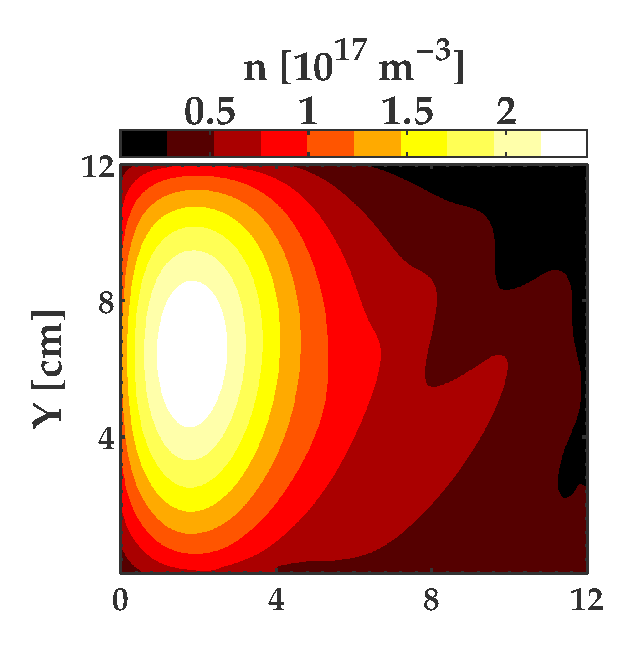
\includegraphics[height=6cm]{figures/4-PegasesCarteDensiteVarBias1.eps}}
    \subfigure[]{\label{4-PegasesCarteDensiteVarBias2}
    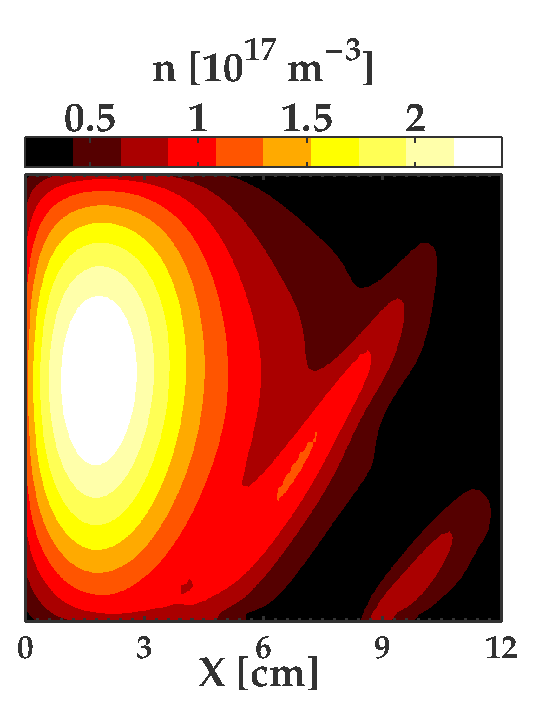
\includegraphics[height=6cm]{figures/4-PegasesCarteDensiteVarBias2.eps}}
    \subfigure[]{\label{4-PegasesCarteDensiteVarBias3}
    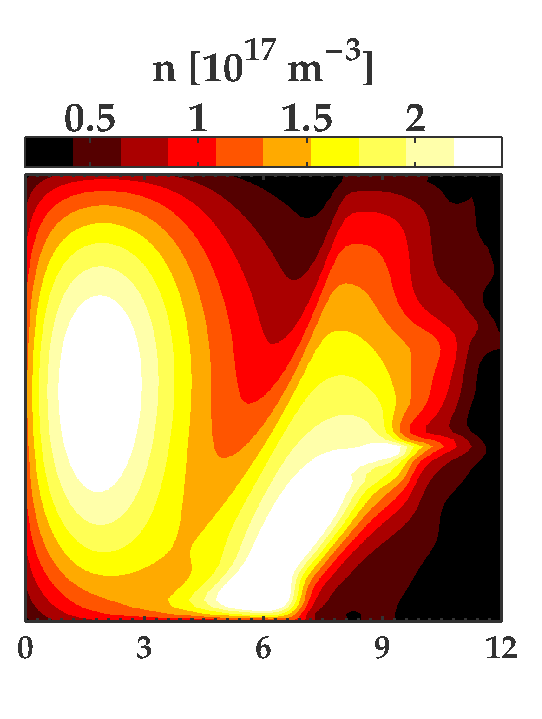
\includegraphics[height=6cm]{figures/4-PegasesCarteDensiteVarBias3.eps}}
    \caption{Cartes de densité\subref{4-PegasesCarteDensiteVarBias1}~, de
    potentiel\subref{4-PegasesCarteDensiteVarBias2}~ et de
    température\subref{4-PegasesCarteDensiteVarBias3}}
    \label{pandas}
\end{figure}

a

\begin{figure}[htbp]
  \centering
    \subfigure[]{\label{4-PegasesCarteDensiteVarBias4}
    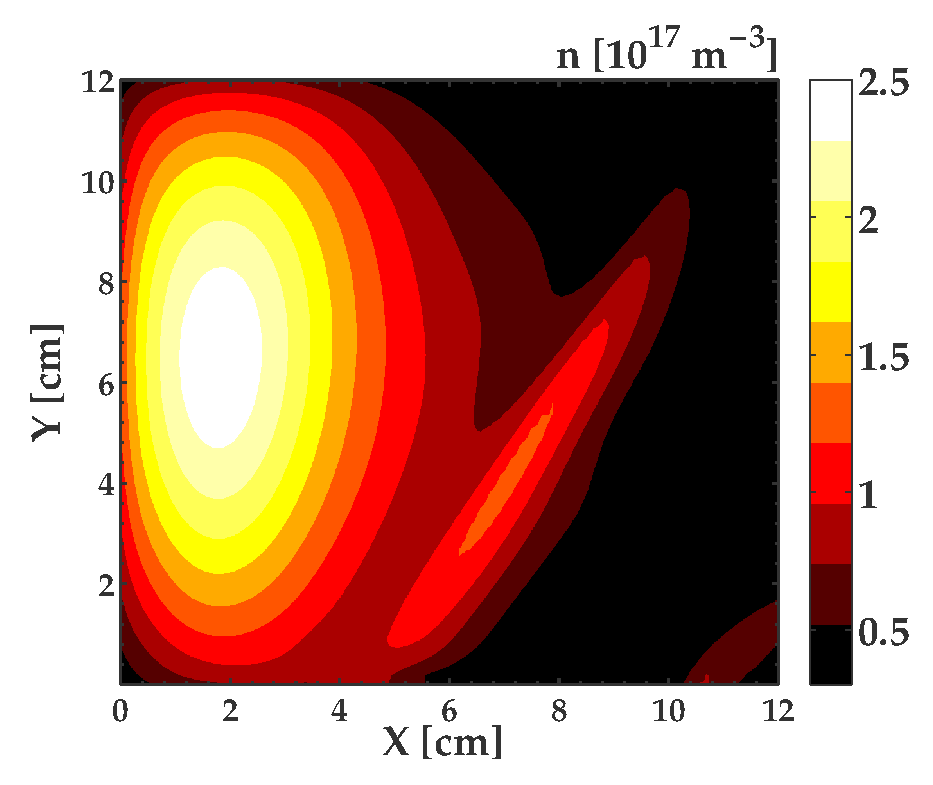
\includegraphics[height=5cm]{figures/4-PegasesCarteDensiteVarBias4.eps}}
    \subfigure[]{\label{4-PegasesCarteViSurTeVarBias}
    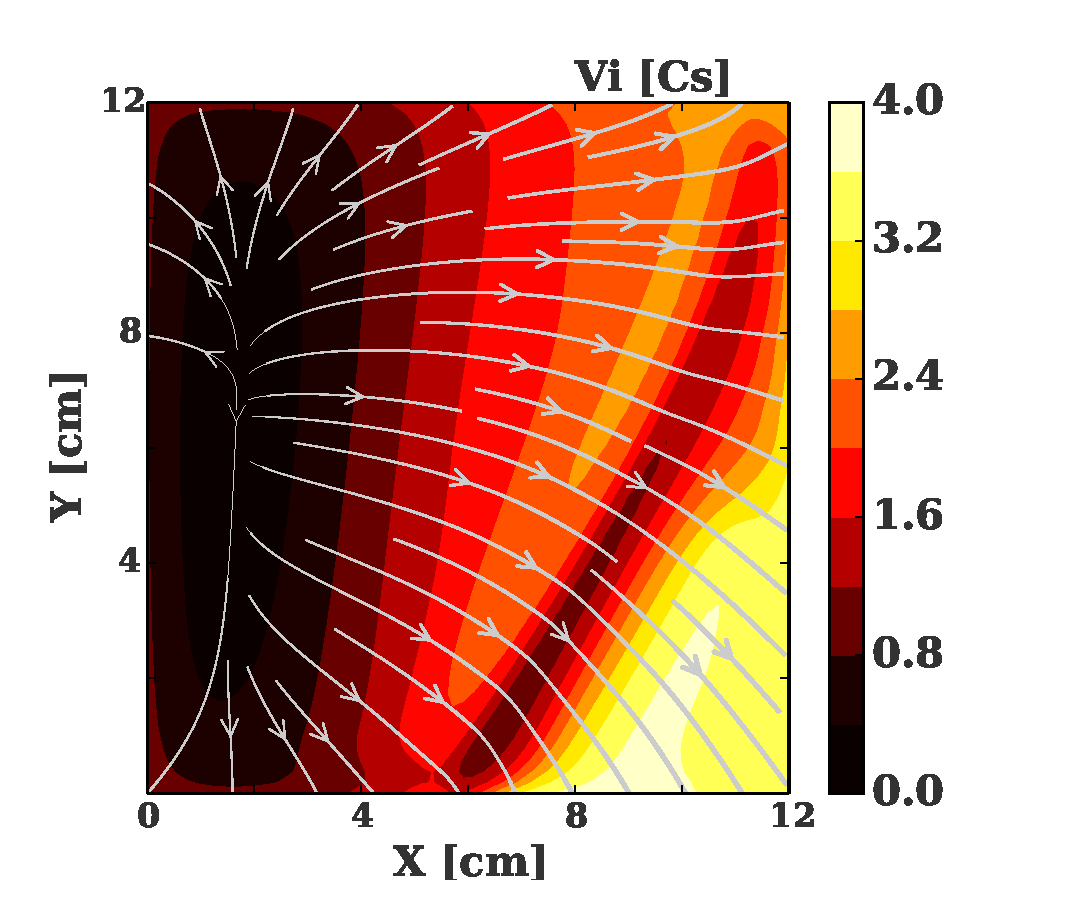
\includegraphics[height=5cm]{figures/4-PegasesCarteViSurTeVarBias.eps}}
    \caption{Cartes de densité\subref{4-PegasesCarteDensiteVarBias1}~, de
    potentiel\subref{4-PegasesCarteDensiteVarBias2}}
    \label{pandas}
\end{figure}
	
	a
	
	\subsubsection{Instabilité liée au gradient de densité}
	\begin{figure}[htbp]
  \centering
    \subfigure[]{\label{4-PegasesCarteDensiteVarBias5}
    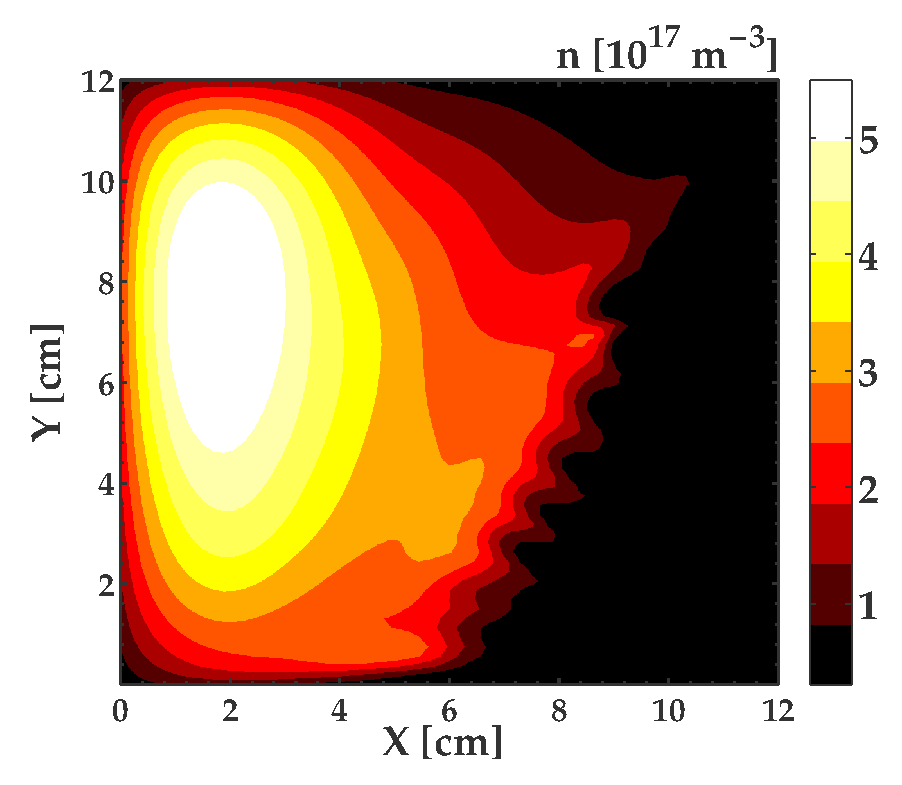
\includegraphics[height=5cm]{figures/4-PegasesCarteDensiteVarBias5.eps}}
    \subfigure[]{\label{4-PegasesCarteDensiteVarBias6}
    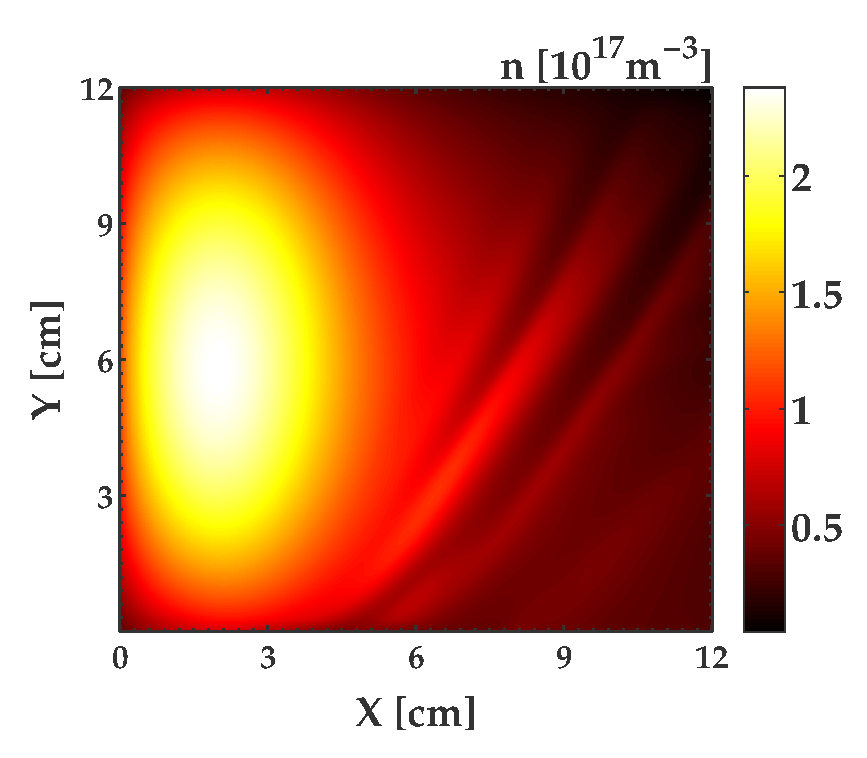
\includegraphics[height=5cm]{figures/4-PegasesCarteDensiteVarBias6.eps}}
    \caption{Cartes de densité\subref{4-PegasesCarteDensiteVarBias5}~, de
    potentiel\subref{4-PegasesCarteDensiteVarBias6}}
    \label{pandas}
\end{figure}
	
\section{Colonne de plasma magnétisée - CYBELE}
a

\begin{figure}[htbp]
  \centering
    \subfigure[]{\label{4-cybelePhoto}
    \includegraphics[height=12cm]{figures/4-cybelePhoto.png}}
    \subfigure[]{\label{4-cybeleSchema}
    \includegraphics[height=10cm]{figures/4-cybeleSchema.png}}
    \caption{Cartes de densité\subref{4-cybelePhoto}~, de
    potentiel\subref{4-cybeleSchema}}
    \label{pandas}
\end{figure}	

a

\begin{figure}[htbp]
\centering
\includegraphics[width=0.8\textwidth]{figures/4-magnetizedColumn.jpg}
{\caption{Transport des ions et des électrons dans une colonne de
plasma\parencite{Rozhansky}.}
\label{4-magnetizedColumn}}
\end{figure}

a

\begin{figure}[htbp]
\centering
\includegraphics[width=0.8\textwidth]{figures/4-cybeleSimDomain.png}
{\caption{Le domaine de simulation est le plan perpendiculaire au champ
magnétique.}
\label{4-cybeleSimDomain}}
\end{figure}

a

\begin{figure}[htbp]
  \centering
    \subfigure[]{\label{4-CybeleCarteDensiteBase}
    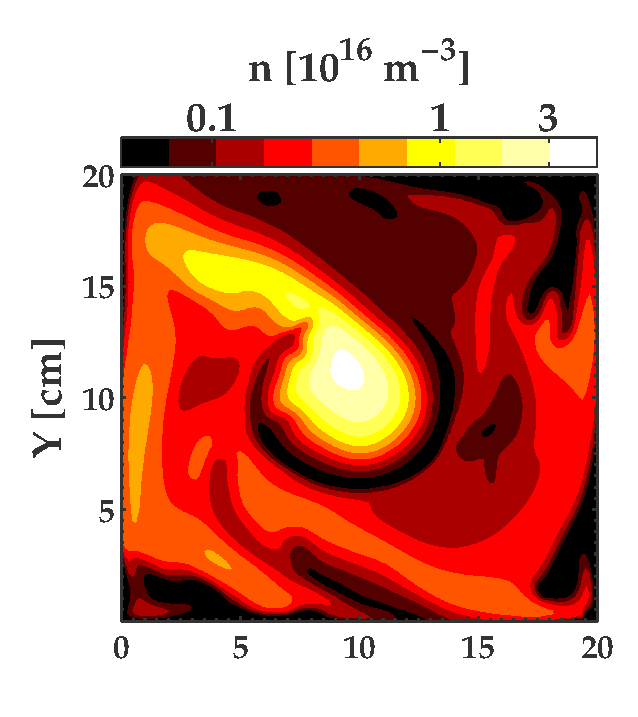
\includegraphics[height=5.5cm]{figures/4-CybeleCarteDensiteBase.eps}}
    \subfigure[]{\label{4-CybeleCartePotentielBase}
    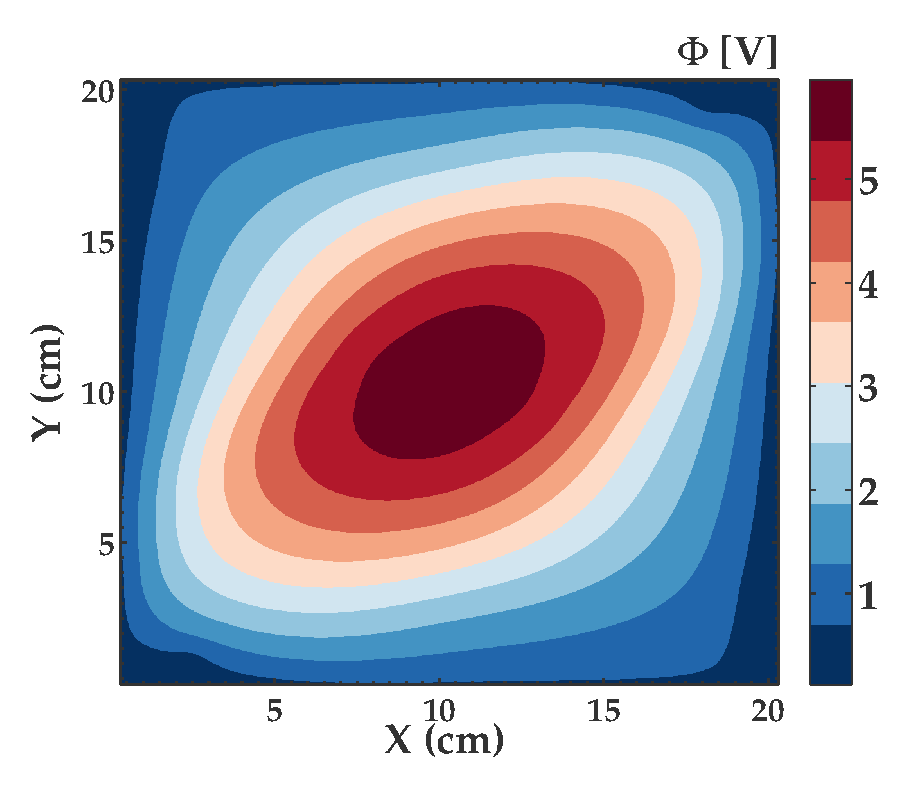
\includegraphics[height=5.5cm]{figures/4-CybeleCartePotentielBase.eps}}
    \subfigure[]{\label{4-CybeleCarteTemperatureBase}
    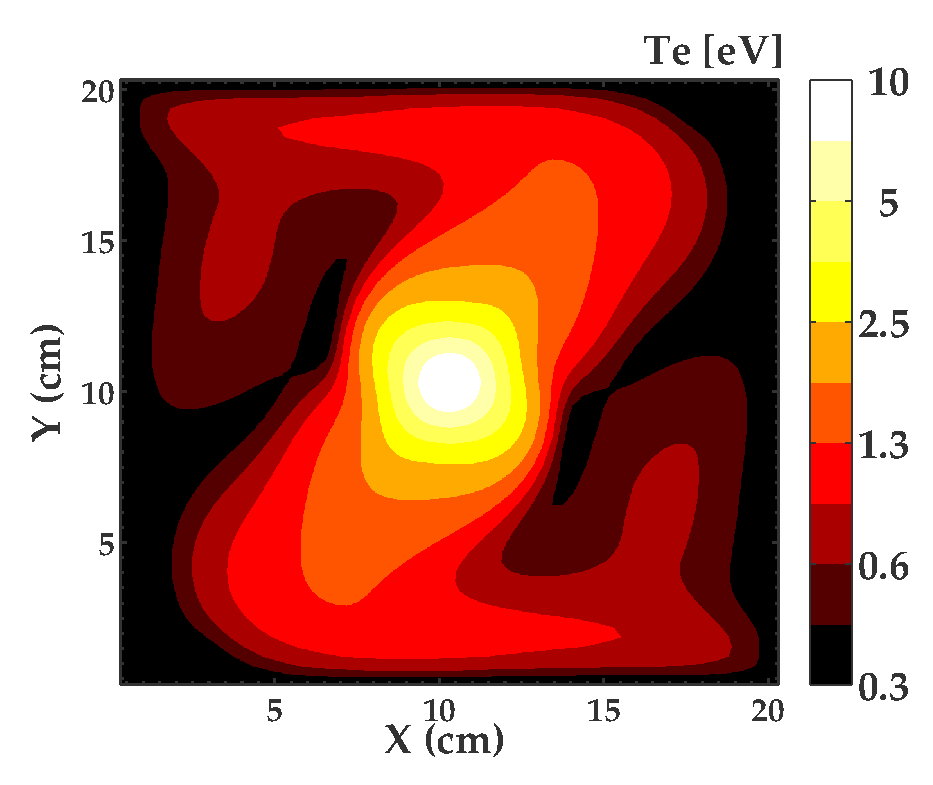
\includegraphics[height=5.5cm]{figures/4-CybeleCarteTemperatureBase.eps}}
    \caption{Cartes de densité \subref{4-CybeleCarteDensiteBase}~, de
    potentiel \subref{4-CybeleCartePotentielBase}~ et de
    température \subref{4-CybeleCarteTemperatureBase}}
    \label{pandas}
\end{figure}

a

\begin{figure}[htbp]
\centering
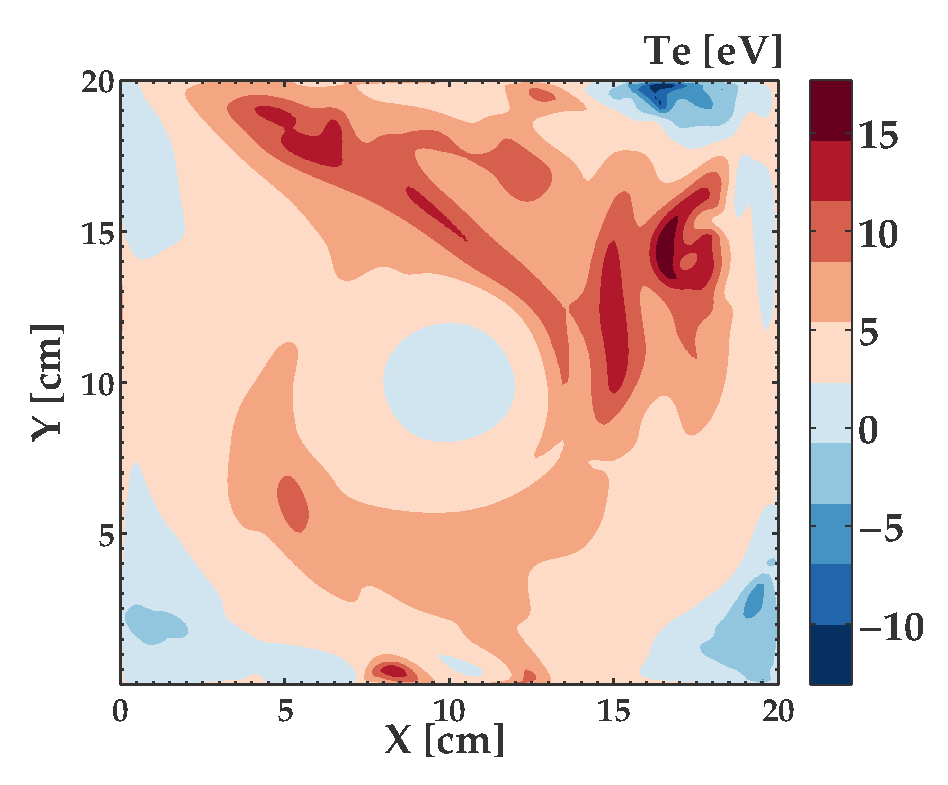
\includegraphics[width=0.8\textwidth]{figures/4-CybeleCartePhiSurTeBase.eps}
{\caption{Carte du potentiel électrostatique rapporté à la température
électronique.}
\label{4-CybeleCartePhiSurTeBase}}
\end{figure}

a

\begin{figure}[htbp]
  \centering
    \subfigure[]{\label{4-CybeleCarteFluxIBase}
    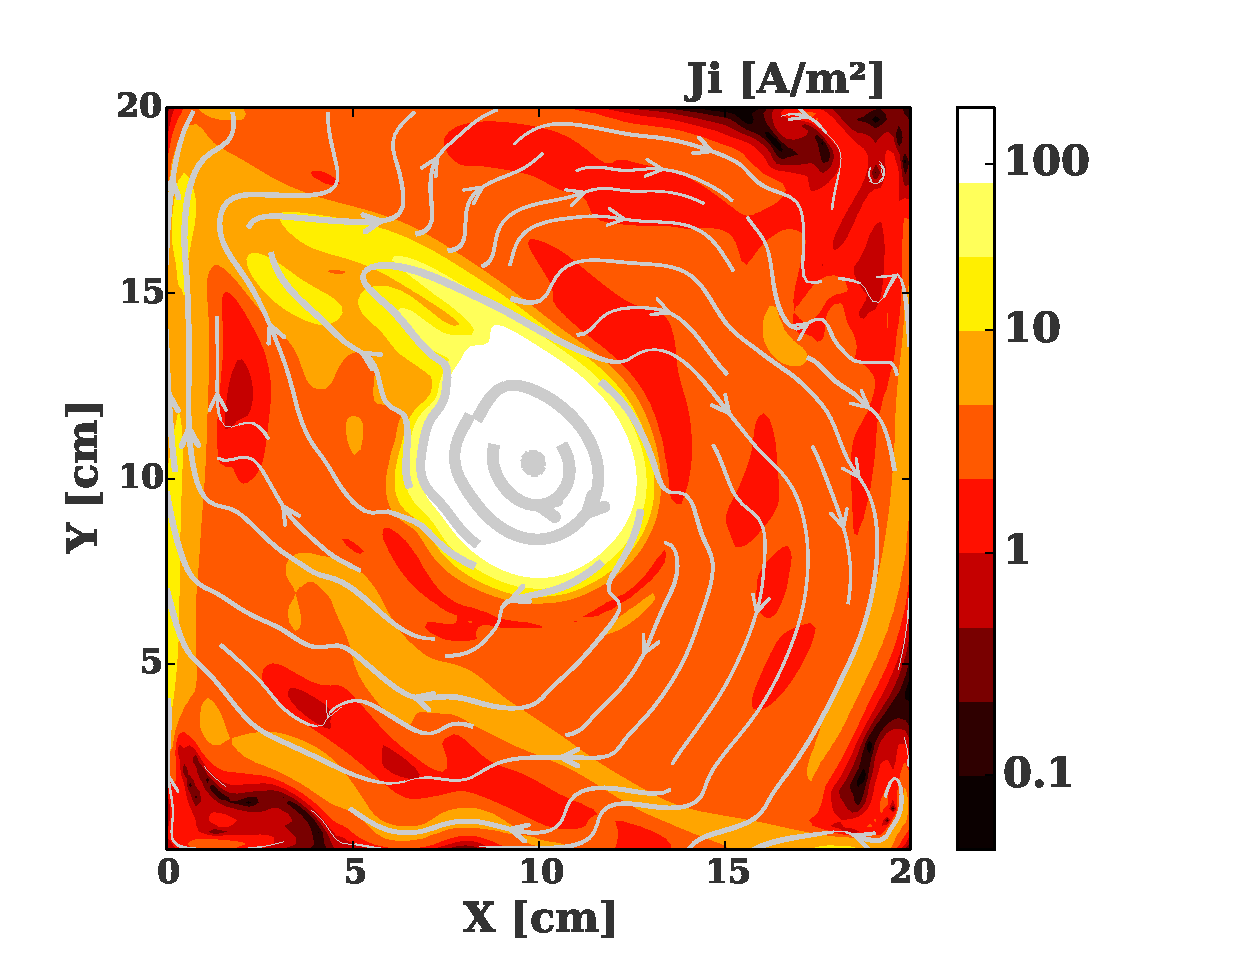
\includegraphics[height=5.5cm]{figures/4-CybeleCarteFluxIBase.eps}}
    \subfigure[]{\label{4-CybeleCarteFluxEBase}
    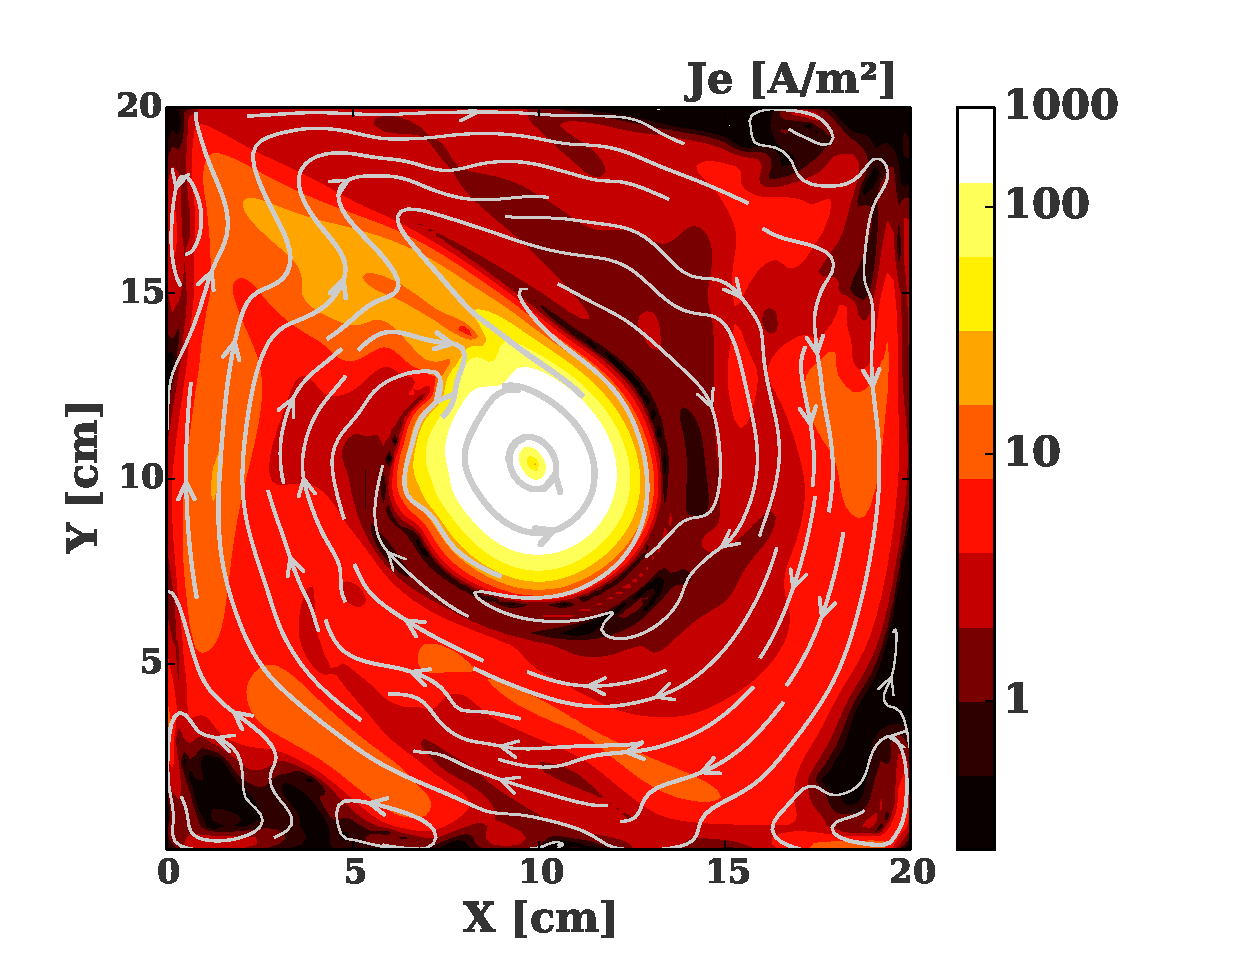
\includegraphics[height=5.5cm]{figures/4-CybeleCarteFluxEBase.eps}}
    \caption{Cartes de densité \subref{4-CybeleCarteFluxEBase}~ et de
    température \subref{4-CybeleCarteCourant}}
    \label{pandas}
\end{figure}

a

\subsection{Le transport transverse magnétisé}

\begin{figure}[htbp]
  \centering
    \subfigure[]{\label{4-CybeleVarMag1}
    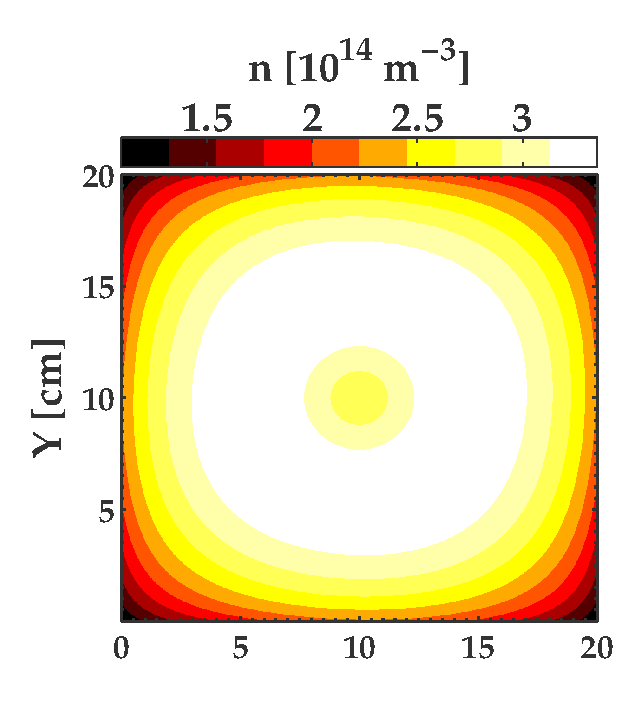
\includegraphics[height=5.5cm]{figures/4-CybeleVarMag1.eps}}
    \subfigure[]{\label{4-CybeleVarMag2}
    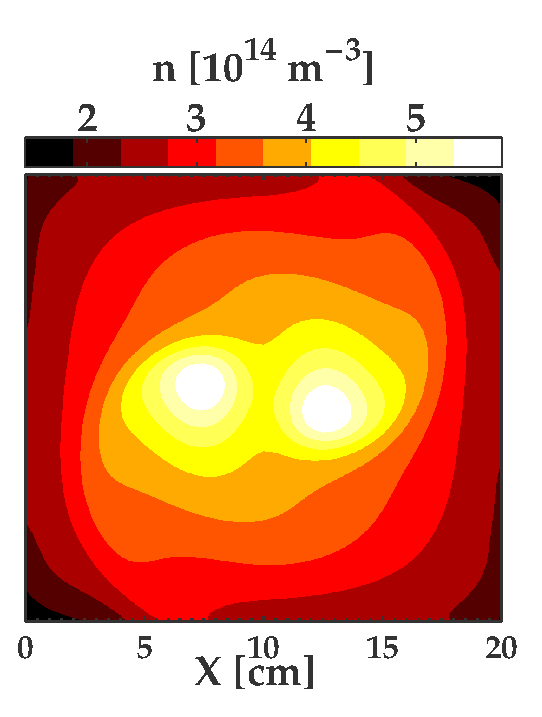
\includegraphics[height=5.5cm]{figures/4-CybeleVarMag2.eps}}
    \subfigure[]{\label{4-CybeleVarMag3}
    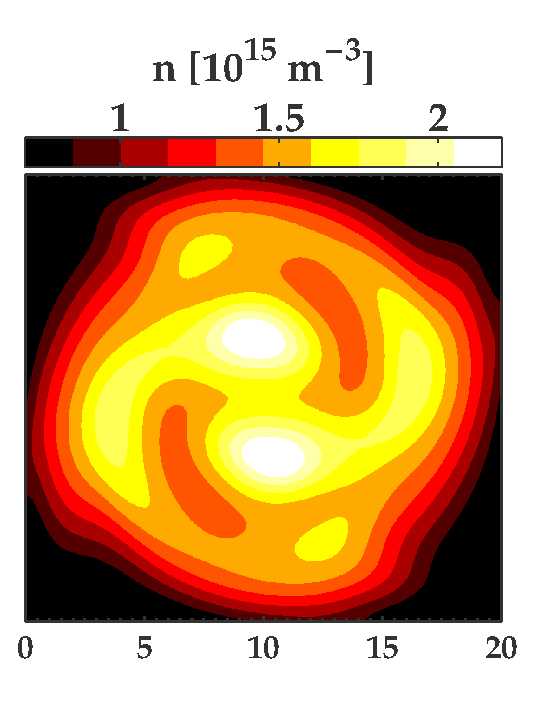
\includegraphics[height=5.5cm]{figures/4-CybeleVarMag3.eps}}
    \caption{Cartes de densité à 1G\subref{4-CybeleVarMag1}~, 4G
    \subref{4-CybeleVarMag2}~ et 15G \subref{4-CybeleVarMag3}}
    \label{pandas}
\end{figure}

a

\begin{figure}[htbp]
  \centering
    \subfigure[]{\label{4-CybeleVarMag4}
    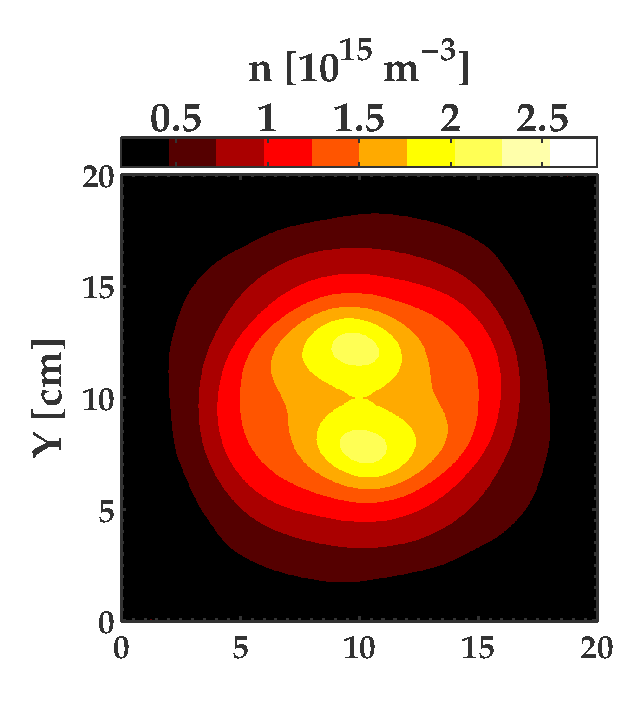
\includegraphics[height=5.5cm]{figures/4-CybeleVarMag4.eps}}
    \subfigure[]{\label{4-CybeleVarMag5}
    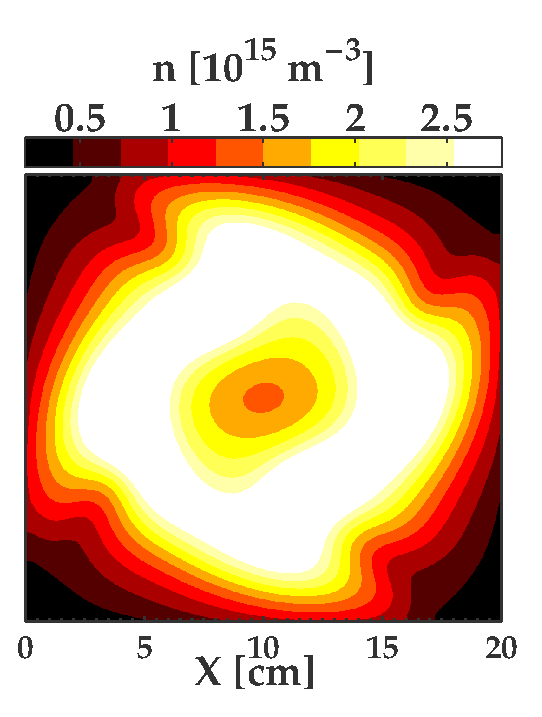
\includegraphics[height=5.5cm]{figures/4-CybeleVarMag5.eps}}
    \subfigure[]{\label{4-CybeleVarMag6}
    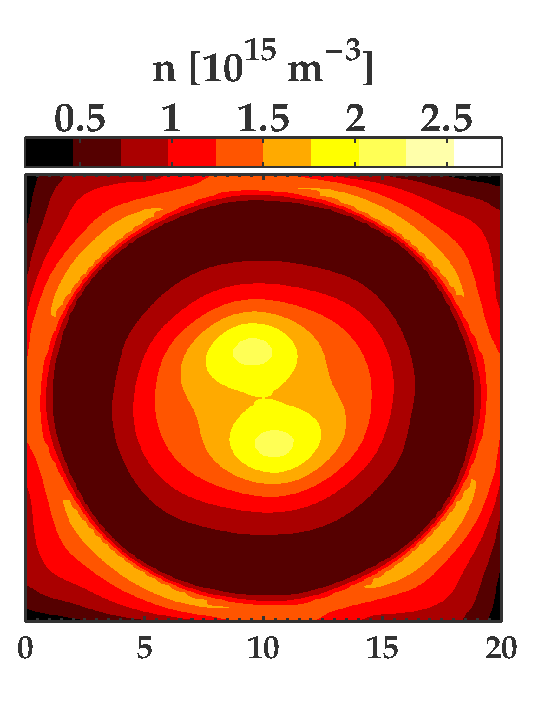
\includegraphics[height=5.5cm]{figures/4-CybeleVarMag6.eps}}
    \caption{Cartes de densité à 20G\subref{4-CybeleVarMag4}~, de
    potentiel \subref{4-CybeleVarMag5}~ et de
    température \subref{4-CybeleVarMag6}}
    \label{pandas}
\end{figure}

a

\begin{figure}[htbp]
\centering
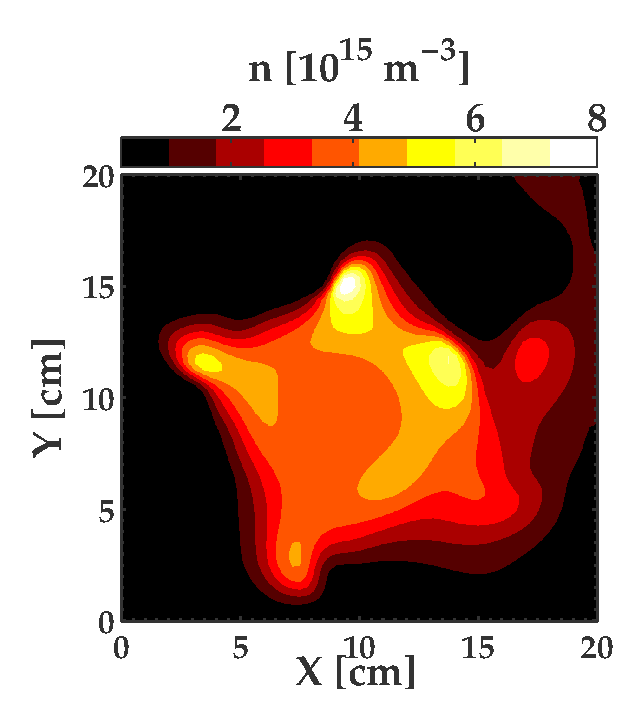
\includegraphics[width=0.5\textwidth]{figures/4-CybeleVarMag8.eps}
{\caption{Carte de densité à 35G.}
\label{4-CybeleVarMag8}}
\end{figure}

a

\begin{figure}[htbp]
  \centering
    \subfigure[]{\label{4-CybeleVarMag9}
    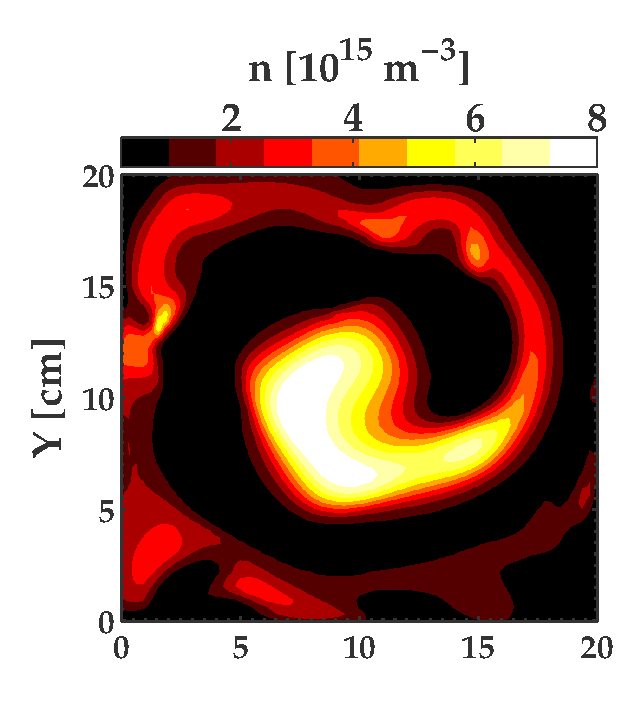
\includegraphics[height=5.5cm]{figures/4-CybeleVarMag9.eps}}
    \subfigure[]{\label{4-CybeleVarMag10}
    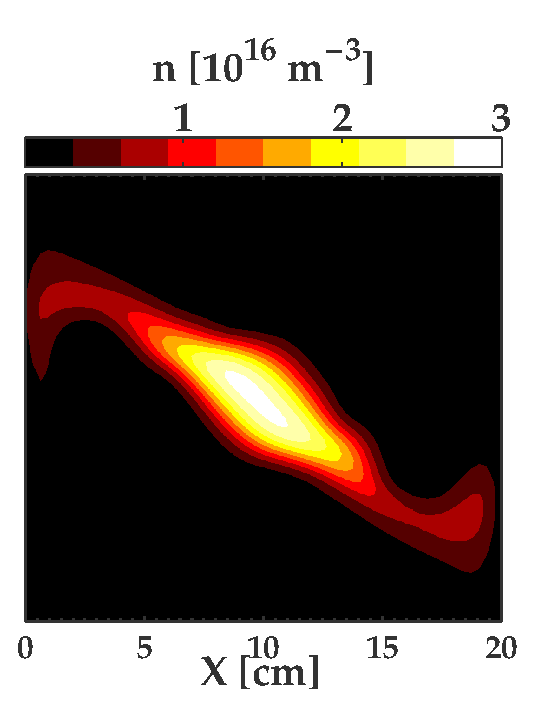
\includegraphics[height=5.5cm]{figures/4-CybeleVarMag10.eps}}
    \subfigure[]{\label{4-CybeleVarMag11}
    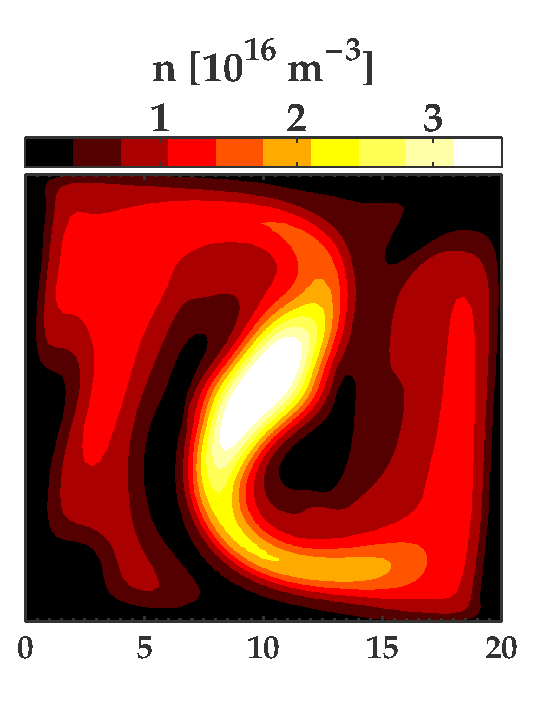
\includegraphics[height=5.5cm]{figures/4-CybeleVarMag11.eps}}
    \caption{Cartes de densité à 80G\subref{4-CybeleVarMag9}~, 130G
    \subref{4-CybeleVarMag10}~ et 170G \subref{4-CybeleVarMag11}}
    \label{pandas}
\end{figure}

a
\begin{table*}
\footnotesize\centering
\ra{1.3}
\begin{tabular}{@{}cccccccccc@{}}\toprule
B&&\multicolumn{3}{c}{Echelles} && \multicolumn{2}{c}{Champs} &&
Rotation\\
\cmidrule{3-5} \cmidrule{7-8} \cmidrule{10-10}
&& $\omega_c$ & $\rho\indice{L}$& $l_{\text{lpm}}$&& $n$ & $T_e$ && 
$\Omega_r$\\
\midrule Phase 1\\
\scriptsize 1-15 &&\scriptsize 10\textsuperscript{4} - 2 10\textsuperscript{5} &
\scriptsize0.1692 &\scriptsize 0.2945 && \scriptsize0.3670 &\scriptsize 0.7187
&& \scriptsize3.1815 \\
Phase 2\\
\scriptsize1-15 &&\scriptsize 10\textsuperscript{4} - 2 10\textsuperscript{5} &
\scriptsize0.1692 &\scriptsize 0.2945 &&\scriptsize 0.3670 &\scriptsize 0.7187
&&\scriptsize 3.1815 \\
Phase 3\\
\scriptsize1-15 &&\scriptsize 10\textsuperscript{4} - 2 10\textsuperscript{5} &
\scriptsize0.1692 &\scriptsize 0.2945 &&\scriptsize 0.3670 &\scriptsize 0.7187
&&\scriptsize 3.1815 \\

\bottomrule
\end{tabular}
\caption{Caption}
\end{table*}
	
	\subsection{Influence du champ magnétique}
	\subsubsection{Influence de la densité de gaz}
\subsection{Polarisation des parois}
		

\section{Plasma de bord de tokamaks}
%\bibliographystyle{apalike}
%\bibliography{biblio}
\end{refsection}
